%! Author = magnus.silverdal
%! Date = 2021-04-22

% Preamble
\documentclass[11pt]{article}

% Packages
\usepackage{amsmath}
\usepackage{graphicx}
\usepackage{fancyhdr}

%data
\title{Studieguide Kapitel 9 Elektricitet}
\author{Magnus Silverdal}
\def\inst{Teknikprogrammet}
\def\typeofdoc{}
\def\course{Fysik 1}
\def\name{Magnus Silverdal}
\def\username{Magnus.Silverdal}
\def\email{\username{}@ga.ntig.se}
\def\graders{Magnus Silverdal}

%Sidhuvud och sidfot
\lfoot{\footnotesize{\name, \\ \email}}
\rfoot{\footnotesize{\today}}
\lhead{\sc\footnotesize\title}
\rhead{\nouppercase{\sc\footnotesize\leftmark}}
\pagestyle{fancy}
\renewcommand{\headrulewidth}{0.2pt}
\renewcommand{\footrulewidth}{0.2pt}

% Document
\begin{document}
    \maketitle
    \section{Beskrivning av kapitlet}
    Målet är att kunna beräkna vad som händer i en elektrisk krets samt att förså hur laddade partiklar rör sig. För att
    göra detta behöver vi förstå sambandet mellan ström, spänning och resistans i en krets. Vi behöver också kunna beräkna kraft och energi
    för laddade partiklar.
    \section{Viktiga begrepp}
    \begin{itemize}
        \item Laddning är en egenskap hos elementarpartiklar, laddning betecknas $Q$ och mäts i Couloumb (förkortat C).
        Elektronen bidrar med laddningen $-1.602 10^{-19} C$ och protonen med laddningen $-1.602 10^{-19} C$. Detta kallas elementarladdningen.
        Laddningen hos ett föremål är summan av alla elektroners och proteners laddning. Med undantag för joner är atomer och molekyler oladdade.
        Laddningen förändras genom att elektroner tillförs eller tas bort.
        \item Den elektriska kraften eller Coulomb-kraften verkar mellan laddade partiklar. Den påminner om garvitationskraften men bestäms av laddningen istället för massan. Om laddningarna har samma tecken repellerar partiklarna,
        d.v.s. kraften är riktad så att partiklarna vill bort från varandra, är laddningarna har olika tecken attraherar partiklarna, kraften vill få partiklarna att röra sig mot varandra. Kraften avtar med kvadraten på avståndet mellan laddningarna.
        \item Om laddningarna, i nästan alla fall syftar vi då på elektronerna, kan röra sig eller inte i ett material beror på om materialet är en ledare eller isolator.
        I en ledare kan elektronerna röra sig mer eller mindre fritt, i en isolator kan de inte röra sig. Metaller och vätskor är exempel på ledare, de flesta andra material leder inte ström.
        Det finns speciella material, halvledare och supraledare, som leder ström åt ett håll eller helt utan motstånd. De kommer vi inte att studera närmare även om de är grunden i nästan all datorteknik.
        \item För att visa hur det elektriska kraftfältet ser ut kan man rita upp den elektriska fältstyrkan $E$. Den definieras av $E = \frac{F}{q}$ där $F$ är hur stor kraft som verkar på en testpartikel med laddningen $q$.
        Fältets riktning ges av pilarna och styrkan av tätheten på, eller avståndet mellan, linjerna.
        \item I en sluten krets, som defineras av att det finns ledare kopplade så att laddningarna kan röra sig från spänningskällans ena pol till den andra, defineras stömmen I som antalet laddningar (i Coulomb) som passerar per sekund. Beteckningen är I och enheten är Ampere.
        \item Fritt fall är när något faller fritt utan luftmotstånd. Gravitationen ger då en konstant acceleration,
        tyngdaccelerationen $g$, som här i Sverige är $9.82 \frac{m}{s^2}$. Eftersom jorden inte är riktigt rund varierar $g$,
        dels beroende på var man befinner sig (högre vid polerna och lägre vid ekvatorn) dels med höjd över havet (högre vid
        havsytan, lägre på hög höjd).
    \end{itemize}
    \section{Viktiga modeller}
    Vid konstant acceleration gäller
    \begin{eqnarray}
        v&=&v_0+at \\
        s&=&v_0 t +  \frac{at^2}{2}
    \end{eqnarray}
    \subsection{Exempeluppgift}
    En skidåkare rör sig med 7,5 m/s. När hon når en
    nerförsbacke börjar hon accelerera med 2,3 m/s2.
    \begin{enumerate}
        \item{a)} Hur lång tid tar det innan hastigheten är 55 km/h?
        \item{b)} Hur långt har skidåkaren färdats efter 3,0
        sekunders färd nerför backen?
        \item{c)} Hur hög hastighet har skidåkaren i slutet av
        backen om den är 59 meter lång och vi kan anta att
        accelerationen är konstant.
    \end{enumerate}
    \section{Sträcka-tid-diagram}
    \begin{figure}[!h]
        \includegraphics[width=\textwidth]{../images/chapter3/DistTime.png}
        \caption{Sträcka-tid diagram. Källa: Impuls Fysik 1}
    \end{figure}
    \clearpage
    \section{Hastighet-tid-diagram}
    \begin{figure}[!h]
        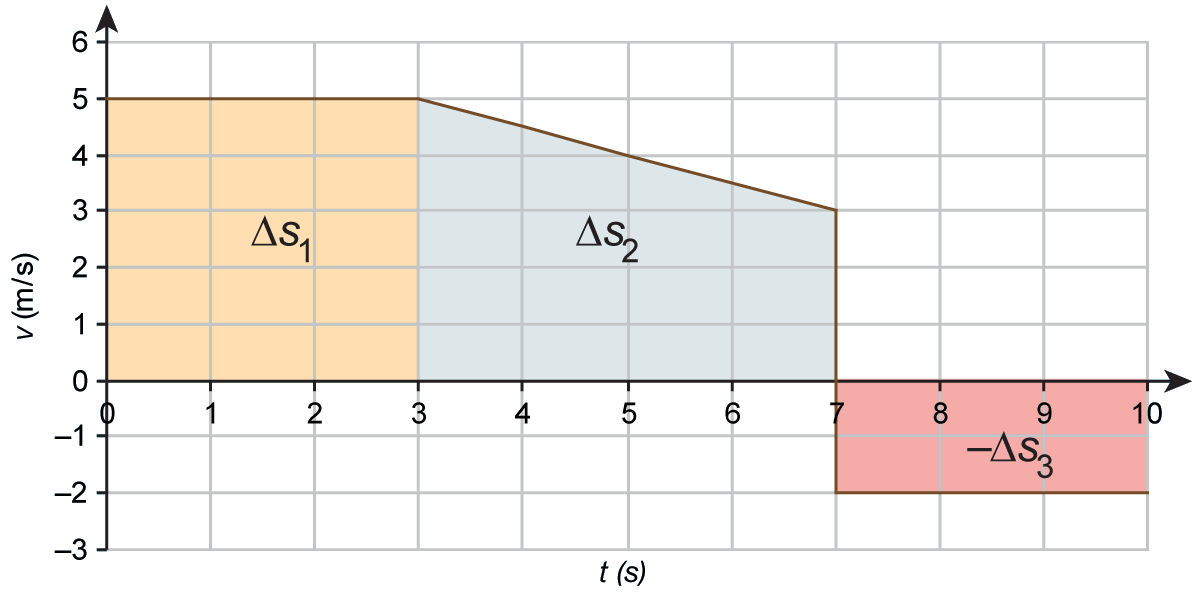
\includegraphics[width=\textwidth]{../images/chapter3/velocityTime.png}
        \caption{Hastighet-tid diagram. Källa: Impuls Fysik 1}
    \end{figure}
    Accelerationen är lutningen på kurvan, sträckan är arean under grafen. Observera att negativ sträcka betyder att
    föremålet rör sig tillbaka mot noll-punkten.
    \begin{figure}[!h]
        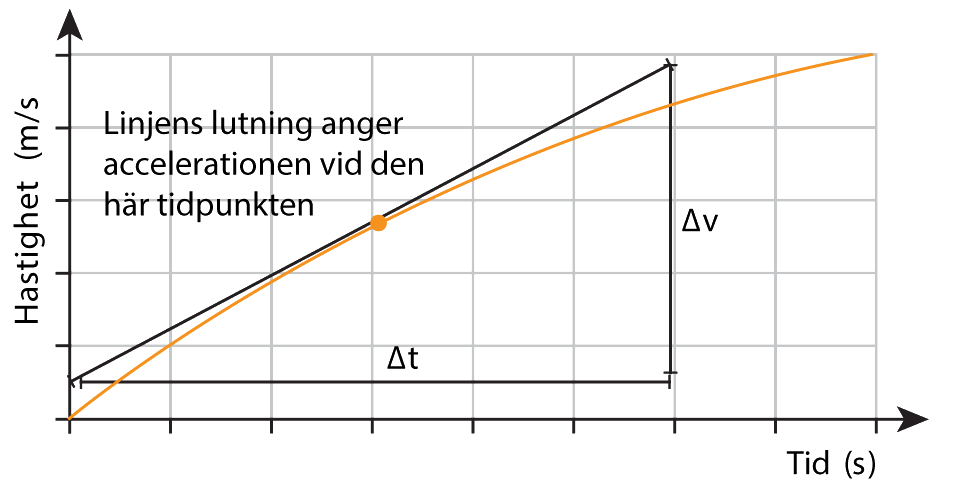
\includegraphics[width=0.5\textwidth]{../images/chapter3/velocityTimeAcceleration.png}
        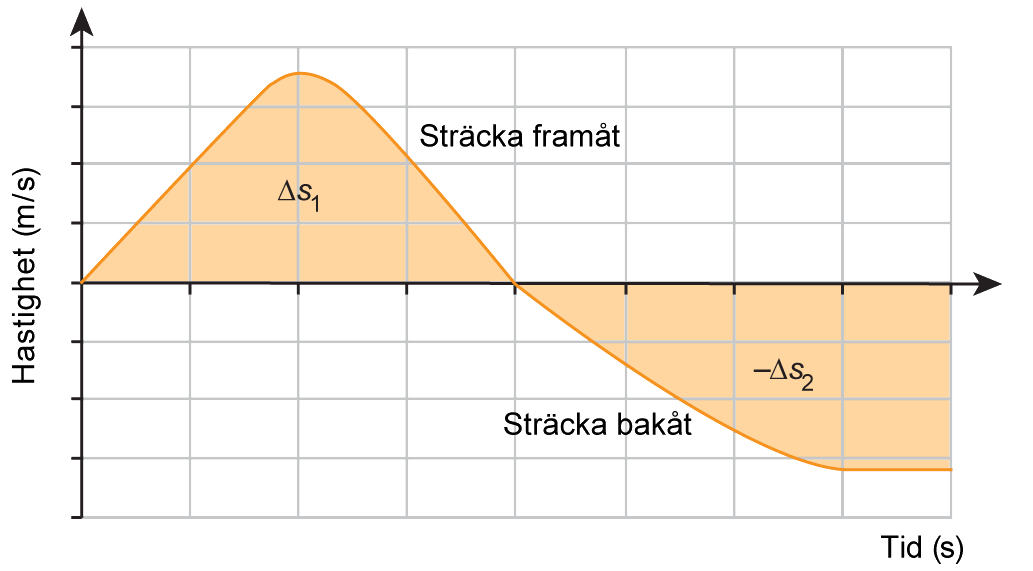
\includegraphics[width=0.5\textwidth]{../images/chapter3/velocityTimeDist.png}
        \caption{Hastighet-tid diagram. Källa: Impuls Fysik 1}
    \end{figure}
    \clearpage
    \section{Acceleration-tid-diagram}
    \begin{figure}[!h]
        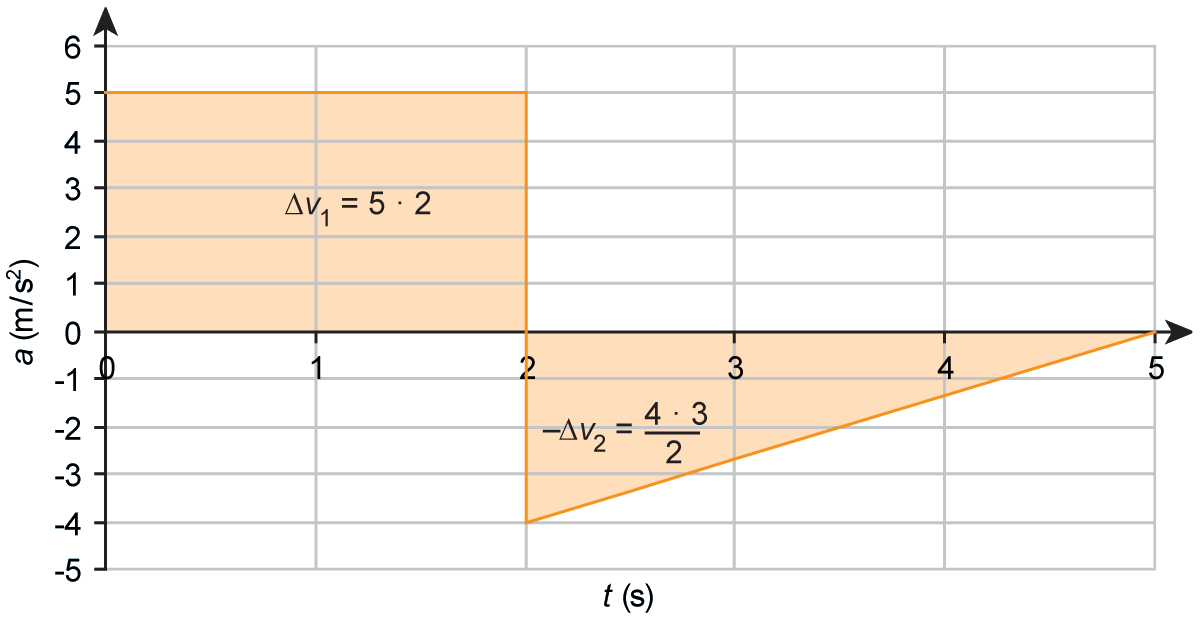
\includegraphics[width=\textwidth]{../images/chapter3/accelerationTime.png}
        \caption{Acceleration-tid diagram. Källa: Impuls Fysik 1}
    \end{figure}
    Förändringen av hastighet är arean under grafen.
    \clearpage
    \section{Planering}
    \begin{table}[h]
        \begin{tabular}{|l|p{6cm}|p{4cm}|l}
            \hline
            17/9 & Momentanhastighet, medelhastighet och hastighet som vektor. & Sidorna 46-51 & uppgifterna 302-316, lös de jämna uppgifterna bara. \\

            18/9 & Sträcka-tid diagram och hastigheten som kurvans lutning (derivata) & Sidorna 52-55. & uppgifterna 318-326 \\

            23/9 & Acceleration. & Sidorna 56-60, &  uppgifterna 327-338 \\

            24/9 & Hastighet-tid och acceleration-tid-diagram. & Sidorna 61-72, & uppgifterna fram till 349 \\

            25/9 & Rörelse med konstant acceleration. De två viktigaste modellerna v=v0 + a t och s = v0
            t + a t^2 / 2.  & Sidorna 73-77. &  Uppgifterna 350-359. \\

            1/10 & Repetition. & & Uppgifterna 360-391 \\

            2/10 & Kunskapstest. Kapitel 3. Vi lånar tid från programmeringslektionen för att ni inte ska hamna i tidsnöd. & & \\

            \hline
        \end{tabular}
    \end{table}

\end{document}